\documentclass[11pt, oneside]{article}   	% use "amsart" instead of "article" for AMSLaTeX format
\usepackage{geometry,graphicx}
\usepackage{graphicx}
\usepackage{amssymb}
\usepackage{amsthm}
\usepackage{amsmath, multirow}
\geometry{
  top = 23mm,
  left = 18mm, 
  right = 18mm,
  bottom = 25mm,
}
\newcommand\tab[1][1cm]{\hspace*{#1}}
\newcommand\ftab[1][5cm]{\hspace*{#1}}
\newcommand\ttab[1][2cm]{\hspace*{#1}}
\newcommand\tsp[1][0.2cm]{\hspace*{#1}}
\newcommand\htab[1][0.5cm]{\hspace*{#1}}
\usepackage[]{algorithm2e}
\geometry{letterpaper}
\usepackage{titlesec}
\setcounter{secnumdepth}{4}
\renewcommand{\baselinestretch}{1.05}
\titlespacing*{\section}
{0pt}{1.3\baselineskip}{1\baselineskip}
\theoremstyle{definition}
\newtheorem{definition}{Definition}[section]

%\usepackage{parskip}

\graphicspath{ {images/} }

\newtheorem*{theorem}{Theorem}
\newtheorem{lemma}{Lemma}
\newtheorem{sublemma}{Lemma}[section]
%SetFonts

\title{Dijkstra's Algorithm Verification}
\author{Yazhe Feng}
%\date{}							% Activate to display a given date or no date

\begin{document}
\maketitle

\section{Dijkstra's Algorithm}

\subsection{Pseudocode}
Given input graph $g$ and source node $s$ with types:
\\\\
  \tab g : Graph gsize weight\\
  \tab s : Node gsize
\\\\
We denote $(u, v)$ as an edge from node $u$ to $v$, $weight(u, v)$ as the weight of edge $(u, v)$. We define $unexplored$ as the list of unexplored nodes, and $dist$ as the list storing distance from $s$ to each node $n \in g$
\\\\
\tab (initially $unexplored$ contains all nodes in graph $g$)\\
\tab $unexplored : List (Node \tsp gsize)$\\
\tab $unexplored = \{v : v \in g\}$
\\\\
\tab (node value is used to index $dist$, initially distance of all nodes are infinity except 
\\ \tab the source node)\\
\tab $dist : List \tsp weight$ \\
\tab $dist[s] = 0, dist[a] = infinity, \forall a \in g, a \neq s$
\\\\The Dijkstra's Algorithm runs as follows: 
Given graph $g$ and source node $s$, $dist$ stores the distance value from $s$ to all nodes in $g$ calculated by the Dijkstra's algorithm, $dist[v]$ gives the corresponding distance value of $v$ from $s$. We index $unexplored$ and $dist$ by the number of iterations. Specifically, denote $u_i$ as the node being explored at the $i^th$ iteration, and denote $dist_i$, $unexplored_i$ as the value of distance list and unexplored list at the beginning of the $i^{th}$ iteration. Then during each iteration the Dijkstra's Algorithm calculates $dist, unexplored, explored$ as follows:
\\\\
\texttt{
  \tab\tab choose $u_k \in unexplored_k$ and $\forall u' \in unexplored_k, dist_k[u_k] \leq dist_k[u']$ \\
  \tab\tab $unexplored_{k+1} = unexplored_k - \{u_k\}$                    \\
  \tab\tab $\forall v \in g$, \\
  \tab\[
        dist_{k+1}[v] = \left.
       \begin{cases} 
          min(dist_k[v], (dist_k[u_k] + weight(u_k,v))), & (u_k,v) \in g \\ 
          dist_k[v] & otherwise 
        \end{cases}
        \right\}
      \]
  \tab\tab \\
  % \tab while (unexplored is not Nil)  \\
  % \tab$\{$ \\
  % \tab\tab choose $u \in unexplored_k$ s.t.$\forall u' \in unexplored_k, dist_k[u] \leq dist_k[u']$     \\
  % \tab\tab let $unexplored_{k+1} = unexplored_k - u$\\
  % \tab\tab for($\forall v \in g$, $(u_k, v) \in g$) $\{$                                 \\
  % \tab\tab\tab  $dist_{k+1}[v] = min(dist_k[v], dist_k[u] + weight(u, v))$                  \\
  % \tab\tab $\}$ \\
  % \tab\tab for($\forall v' \in g$ s.t. v' is not a neighbor of u, i.e. $(u, v') \notin g$) $\{$     \\
  % \tab\tab\tab  $dist_{k+1}[v'] = dist_{k}[v'] $                                \\
  % \tab\tab $\}$ \\
  % \tab\tab input the new $unexplored_{k+1}$ and $dist_{k+1}$ to the $(k+1)^{th}$ iteration of the while loop \\
  % \tab $\}$ \\
}

\subsection{Assumptions}
\begin{enumerate}
  \item Weight of edges are positive
  \item Distance value can only be zero, infinity, or summation of edge weights
  \item All nodes $n$ and edge $e$ are valid: $n, e \in g$
\end{enumerate}



\section{Definition}
\theoremstyle{definition}
\begin{definition}\textbf{Path}\\
\textit{(We adopt the definition of $path$ presented in the \texttt{Discrete Mathematics with Applications} book by \texttt{SUSANNA S. EPP}.)}
\\\\
A path from node $v$ to $w$ is a finite alternating sequence of adjacent vertices and edges of G, which does not contain any repeated edge or vertex. A path from $v$ to $w$ has the form: 
\begin{center}
 $ve_0v_0e_1v_2....v_{n-1}e_nw$ 
\end{center}
where $e_i$ is an edge in $g$ with endpoints $v_{i-1}, v_i$. We denote the set of paths from $v$ to $w$ as $path(v, w)$.
\end{definition}
\tab
\begin{definition}\textbf{Prefix of Path}\\
Given a path from node $v$ to $w$ : $p(v, w) = ve_0v_0e_1v_2....v_{n-1}e_nw$, the prefix of this $v-w$ path is defined as the subsequence of $p(v, w)$ that starts with $v$ and ends with some node $w' \in p(v, w)$ ($w'$ is a vertex in the sequence $p(v, w)$). 
\end{definition}
\tab
\begin{definition}\textbf{Length of Path} \\
The length of a path $p = ve_0v_0e_1v_2....v_{n-1}e_nw$ is the sum of the weights of all edges in $p$. We write: 
\begin{center}
  $length(p) = \sum weight(e_i), \forall e_i \in p$. 
\end{center} 
\end{definition}
\tab
\begin{definition}\textbf{Shortest Path}\\
Denote $\Delta(s, v)$ as the shortest path from $s$ to $v$, and $\delta(v)$ as the length of $\Delta(s, v)$. $\Delta(s, v)$ must fulfills: 
\begin{center}
$\Delta(s, v) \in path(s, v)$ 
\\
and 
\\
$\forall p' \in path(s, v)$, $\delta(v) = length(\Delta(s, v)) \leq length(p')$
\end{center}
\end{definition}

\section{Proof of Correctness}
\subsection{Proof of Termination}
The inner for loop is guaranteed to terminate as the algorithm goes through each adjacent node exactly once. As the size of list \texttt{unexplored} decreases by one during each iteration of the while loop, the algorithm is guaranteed to terminate. 


\subsection{Proof of Correctness}
Denote $explored$ as the list of nodes in $g$ but not in $unexplored$, i.e., $explored$ stored all nodes whose neighbors have been updated by the algorithm. We index $explored$ by the number of iterations, such that $explored_i$ denotes the value of $explored$ at the beginning of the $i^{th}$ iteration.


\begin{sublemma}
Given any two nodes $v, w$, the prefix of the shortest path $\Delta(v, w)$ is also a shortest path. 
\end{sublemma}
\begin{proof}
We will prove Lemma 3.1 by contradiction. 
\\
Consider any node $q$ in the sequence of $\Delta(v, w)$, we have $\Delta(v, w) = ve_0v_0e_1v_2...v_i q v_j....v_{n-1}e_nw$. Suppose the prefix of $\Delta(v, w)$ from $v$ to $q$, denote as $p(v, q)$, is not the shortest path from $v$ to $q$. Then we know $p(v, q) = ve_0v_0e_1v_2...v_iq$ is a path from $v$ to $q$ and $length(p(v, q)) > length(\Delta(v, q))$. 
\\
Based on the definition of shortest path, we know: 
\\\\
\ftab $length(\Delta(v, w)) \leq length(p), \forall  p \in path(v, w)$
\\\\
Fenote the path after the node $q$ as $p(q, w) = q v_j....v_{n-1}e_nw$, since $\Delta(v, w) = ve_0v_0e_1v_2...v_i q v_j....v_{n-1}e_nw$, then $\Delta(v, w) = p(v, q) + p(q, w)$, and that $length(\Delta(v, w)) = length(p(v, q)) + length(p(q, w))$. Then we have: 
\\\\
\tab$length(\Delta(v, w)) = length(p(v, q)) + length(p(q, w)) \leq length(p), \forall p \in path(v, w)$
\\\\
Since $p(v, q)$ is not the shortest path from $v$ to $q$ by assumption, there exists another $v-w$ path $p'(v, w)$ such that: 
\\\\
\ftab $p'(v, w) \in path(v, w)$\\
\ftab $p'(v, w) = \Delta(v, q) + p(q, w)$ \\ 
\ftab $length(p'(v, w)) = length(\Delta(v, q)) + length(p(q, w))$ \\ 
\ftab\tab\tab\htab\tsp$< length(p(v, q)) + length(p(q, w))$ \\
\ftab i.e. $length(p'(v, w)) < length(\Delta(v, w))$
\\\\
Hence we have reached a contradiction. Thus by the principle of prove by contradiction, for any the prefix $p(v, q)$ of $\Delta(v, w)$ is the shortest path from $v$ to $q$. Lemma 3.1 holds. 
\end{proof}
\tab \\


\begin{sublemma}
After the $n^{th}$ iteration for $n \geq 1$, forall node $v \in explored_{n+1}$, if $dist_{n+1}[v] \neq infinity$, then $dist_{n+1}[v]$ is the length of some $s-v$ path, i.e, $path(s, v) \neq \emptyset$.  
\end{sublemma}
\begin{proof}
We will prove \texttt{Lemma 3.2} by inducting on the number of iterations. 
\\
Let P(n) be: After the $n^{th}$ iteration, $n \geq 1$, for all node $v \in g$, if $dist_{n+1}[v] \neq infinity$, then $dist_{n+1}[v]$ is the length of some $s-v$ path. 
\\
\textbf{Base Case}: We shall show P(1) holds. 
\\
Based on the algorithm, initially $dist_1[s] = 0$ and for all node $v \in g, v \neq s, dist_1[v] = infinity$, then $s$ is the only node whose distance value is not infinity. Based on the definition of path, the path from the source node $s$ to itself is $s$, $path(s, s) = \{s\}$. Hence P(1) holds. 
\\
\textbf{Inductive Hypothesis}: Suppose $\forall i, 1 \leq i \leq k$, P(i) holds. That is, after the $i^{th}$ iteration, $1 \leq i \leq k$, for all nodes $v \in g$, if $dist_{i+1}[v] \neq infinity$, then $dist_{n+1}[v]$ is the length of some $s-v$ path. 
\\
\textbf{Inductive Step}: We shall show P(k+1) holds.
\\
For node $u_{k+1}$ being explored during the $(k+1)^{th}$ iteration, based on the algorithm, $dist_{k+1}[u_{k+1}]$ is calculated as: 
\\\\
\tab\[
        dist_{k+2}[u_{k+1}] = \left.
       \begin{cases} 
          min(dist_{k+1}[u_{k+1}], dist_{k+1}[u_{k+1}] + weight(u_{k+1},u_{k+1})), & (u_{k+1},u_{k+1}) \in g \\ 
          dist_{k+1}[u_{k+1}] & otherwise 
        \end{cases}
        \right\}
      \]
\\\\
Since the distance value from $u_{k+1}$ to itself is $0$, then $dist_{k+2}[u_{k+1}] = dist_{k+1}[u_{k+1}]$, and that $dist_{k+2}[u_{k+1}]$ and $dist_{k+1}[u_{k+1}]$ are the length of the same $s-u_{k+1}$ path if there exists one. 
\\
If $dist_{k+2}[u_{k+1}] \neq infinity$, then $dist_{k+1}[u_{k+1}] = dist_{k+2}[u_{k+1}] \neq infinity$. Since $k \leq k$ and $dist_{k+1}[u_{k+1}] \neq infinity$, then based on the inductive hypothesis, $dist_{k+1}[u_{k+1}]$ is the length of some $s-u_{k+1}$ path, and hence $dist_{k+2}[u_{k+1}]$ is the length of some $s-u_{k+1}$ path.
\\
Then for all node $v \in g$ other than $u_{k+1}$, there are two cases: (1) $(u_{k+1}, v) \in g$; (2) $u_{k+1}$ does not have an edge to $v$. We will prove P(k+1) holds in both cases separately. 
\\\\
\texttt{Case (1): $(u_{k+1}, v) \in g$}
\\
Based on the algorithm, as $(u_{k+1}, v) \in g$, $dist_{k+2}[v] = min(dist_{k+1}[v], dist_{k+1}[u_{k+1}] + weight(u_{k+1}, v))$. 
\begin{itemize}
  \item If $dist_{k+1}[v] < dist_{k+1}[u_{k+1}] + weight(u_{k+1}, v)$, then $dist_{k+2}[v] = dist_{k+1}[v]$. Then if $dist_{k+2}[v] \neq infinity$, we have $dist_{k+1}[v] \neq infinity$, and that $dist_{k+2}[v]$ and $dist_{k+1}[v]$ are the length of the same $s-v$ path if there exists one. Since $dist_{k+1}[v] \neq infinity$, the inductive hypothesis implies that $dist_{k+1}[v]$ is the length of some $s-v$ path, hence $dist_{k+2}[v]$ is the length of some $s-v$ path. P(k+1) holds. 

  \item If $dist_{k+1}[v] \geq dist_{k+1}[u_{k+1}] + weight(u_{k+1}, v)$, then $dist_{k+2}[v] = dist_{k+1}[u_{k+1}] + weight(w, v)$. If $dist_{k+2}[v] \neq infinity$, then it follows that $dist_{k+1}[u_{k+1}] = dist_{k+2}[v] - weight(u_{k+1}, v) \neq infinity$. Then the inductive hypothesis implies that $dist_{k+1}[u_{k+1}]$ must be the length of some $s-u_{k+1}$ path, denote as $p(s, u_{k+1})$. Since there is an edge $(u_{k+1}, v) \in g$, then $dist_{k+2}[v] = dist_{k+1}[u_{k+1}] + weight(u_{k+1}, v)$ must be the length of the $s-v$ path through $u_{k+1}$. P(k+1) holds. 
\end{itemize}
Hence P(k+1) holds under under \texttt{Case(1)}. 
\\\\
\texttt{Case (2): $u_{k+1}$ does not have an edge to $v$}
\\
Under this case, our algorithm indicates that $dist_{k+2}[v] = dist_{k+1}[v]$, and that $dist_{k+1}[v]$ and $dist_{k+2}[v]$ are the length of the same $s-v$ path if there exists one. If $dist_{k+1}[v] = dist_{k+2}[v] \neq infinity$, then based on the inductive hypothesis, $dist_{k+1}[v]$ is the length of some $s-v$ path, and hence $dist_{k+2}[v]$ is the length of some $s-v$ path. P(k+1) holds under \texttt{Case(2)}. 
\\\\
We have proved P(k+1) holds for $u_{k+1}$ and both cases for all nodes $v \in g$ other than $u_{k+1}$. Hence by the principle of prove by induction, P(n) holds. Thus \texttt{\texttt{Lemma 3.2}} holds. 
\end{proof}
\tab\\ 



\begin{sublemma}
For any node $v \in g$, if after the $i^{th}$ iteration, $dist_{i+1}[v] = \delta(v)$, then for each proceeding $j^{th}$ iteration, $j > i$, $dist_{j+1}[v] = dist_{i+1}[v] = \delta(v)$. 
\end{sublemma}
\begin{proof}
We will prove \texttt{Lemma 3.3} by induction on the number iterations after the $i^{th}$ iteration. 
\\
Let P(n) be: For any node $v \in g$, if after the $i^{th}$ iteration, $dist_{i+1}[v] = \delta(v)$, then for the $(i+n)^{th}$ iteration, $n \geq 1$, $dist_{i+n+1}[v] = dist_{i+1}[v] = \delta(v)$
\\
\textbf{Base Case}: We shall show P(1) holds. 
\\
During the $(i+1)^{th}$ iteration, suppose $u_{i+1}$ is the node being explored, then $dist_{i+2}[v]$ is calculated as: 
\\\\
\tab\[
        dist_{i+2}[v] = \left.
       \begin{cases} 
          min(dist_{i+1}[v], dist_{i+1}[u_{i+1}] + weight(u_{i+1}, v)), & (u_{i+1}, v)) \in g \\ 
          dist_{i+1}[v] & otherwise 
        \end{cases}
        \right\}
      \]
\\\\
If $(u_{i+1}, v)) \in g $, then if $dist_{i+1}[u_{i+1}]$ is the length of some $s-u_{i+1}$ path, then $(dist_{i+1}[u_{i+1}] + weight(u_{i+1}, v))$ is the length of some $s-v$ path. Since $dist_{i+1}[v] = \delta(v)$, then based on the definition of shortest path, $dist_{i+1}[v] \leq dist_{i+1}[u_{i+1}] + weight(u_{i+1}, v)$, and hence $dist_{i+2}[v] = dist_{i+1}[v] = \delta(v)$. 
\\
If $u_{i+1}$ does not have an edge to $v$, then $dist_{i+2}[v] = dist_{i+1}[v] = \delta(v)$. 
\\
Hence in either cases, $dist_{i+2}[v] = dist_{i+1}[v] = \delta(v)$. P(1) holds. 
\\\\
\textbf{Inductive Hypothesis}: Suppose P(k) holds, that is, if after the $i^{th}$ iteration, $dist_{i+1}[v] = \delta(v)$, then for the $(i+k)^{th}$ iteration, $n \geq 1$, $dist_{i+k+1}[v] = dist_{i+1}[v] = \delta(v)$. 
\\\\
\textbf{Inductive Step}: We shall show P(k+1) holds. 
\\
For the node $u_{i+k+1}$ being explored during the $(i+k+1)^{th}$ iteration, there are two cases: (1) $(u_{i+k+1}, v) \in g$; (2) $u_{i+k+1}$ does not have an edge to $v$. We will show that P(k+1) holds under both cases separately. 
\\
\texttt{Case 1: $(u_{i+k+1}, v) \in g$}
\\
If $u_{i+k+1}$ has an edge to $v$, then based on the algorithm, for $dist_{i+k+2}[v]$, we have: 
\\\\
  \tab $dist_{i+k+2}[v] = min(dist_{i+k+1}[v], dist_{i+k+1}[u_{i+k+1}] + weight(u_{i+k+1}, v))$
\\\\
Since based on our inductive hypothesis, $dist_{i+k+1}[v] = dist_{i+1}[v] = \delta(v)$, then if $dist_{i+k+1}[u_{i+k+1}] $ is the length of some $s-u_{i+k+1}$ path, then $(dist_{i+k+1}[u_{i+1}] + weight(u_{i+k+1}, v))$ is the length of some $s-v$ path, and hence $dist_{i+k+1}[v] = \delta(v) \leq (dist_{i+k+1}[u_{i+1}] + weight(u_{i+k+1}, v))$. Then: 
\\\\
 \tab $dist_{i+k+2}[v] = min(dist_{i+k+1}[v], dist_{i+k+1}[u_{i+k+1}] + weight(u_{i+k+1}, v)) \\
 \tab\tab\tab = dist_{i+k+1}[v]\\
 \tab\tab\tab = dist_{i+1}[v] = \delta(v)$
\\\\
P(k+1) holds under \texttt{Case 1}. 
\\
\texttt{Case 2: $u_{i+k+1}$ does not have an edge to $v$}
\\
Since $u_{i+k+1}$ does not have an edge to $v$, then $dist_{i+k+2}[v] = dist_{i+k+1}[v]$. Based on the inductive hypothesis, $dist_{i+k+1}[v] = dist_{i+1}[v] = \delta(v)$. then $dist_{i+k+2}[v] = dist_{i+1}[v] = \delta(v)$. P(k+1) holds for \texttt{Case (2)}. 
\\
Thus P(k+1) holds. By the principle of prove by induction, P(n) holds. \texttt{Lemma 3.3} proved. 

\end{proof}



\begin{sublemma}
Assume $g$ is a connected graph, that the source node $s$ has a path to every node in $g$. After the $n^{th}$ iteration of the algorithm for $n \geq 1$, forall node $v \in explored_{n+1}$, we have:
\begin{enumerate}
  \item $\delta(v) \leq \delta(v')$, $\forall v' \in unexplored_{n+1}$.
  \item $dist_{n+1}[v] = \delta(v)$
\end{enumerate}
\end{sublemma}
\begin{proof}
We will prove \texttt{Lemma 3.4} by inducting on the number of iterations. 
\\
Let P(n) be: After the $n^{th}$ iteration of the algroithm for $n \geq 1$, forall node $w \in explored_{n+1}$: (1) $\delta(w) \leq \delta(w')$, $\forall w' \in unexplored_{n+1}$; (2) $dist_{n+1}[w] = \delta(w)$. %; and (3) $dist_m[v] = dist_n[v] = \delta(v)$ for all proceeding $m^{th}$ iteration of the algorithm, $m > n$. 
\tab\\\\
\textbf{Base Case}: We shall show P(1) holds \\
Based on the algorithm, during the first iteration, the node with minimum distance value is the source node $s$ with $dist_1[s] = 0$. Hence during the first iteration, only $s$ is removed from $unexplored_1$ and added to $explored_2$. Since all edge weights are non-negative, then the shortest distance value from $s$ to $s$ is indeed $0$, hence $dist_2[s] = 0 = \delta(s)$ and $\delta(s) \leq \delta(v')$, $\forall v' \in unexplored_2$. 
% \\
% Since during proceeding iterations, the algorithm only updates the distance value of $s$ when there exists some node $w$ such that $dist_i[w] + weight(w, s) < dist_1[s]$, but $dist_1[s] = 0$ and all edge weights are non-negative, then there there does not exists such $w$ such that $dist_i[w] + weight(w, s) < dist_1[s]$. Hence the value of $dist_i[s]$ fulfills $dist_i[s] = dist_1[s] = \delta(s, s)$ for all $i > 1$. 
\\
P(1) holds.
\\\\
\textbf{Inductive Hypothesis}: Suppose P(i) is true for all $1 \leq i \leq k$. That is, after the $i^{th}$ iteration forall $1 < i \leq k$, forall node $w \in explored_{i+1}$: (1) $\delta(w) \leq \delta(w')$, $\forall w' \in unexplored_{i+1}$; (2) $dist_{i+1}[w] = \delta(w)$; %and $dist_m[v] = dist_n[v] = \delta(v)$ for all proceeding $m^{th}$ iteration of the algorithm, $m > n$. 
\\\\
\textbf{Inductive Step}: We shall show P(k+1) holds. That is, forall node $w \in explored_{k+2}$, (1) $\delta(w) \leq \delta(w')$, $\forall w' \in unexplored_{k+2}$; (2) $dist_{k+2}[w] = \delta(w)$;
\\
Suppose $u_{k+1}$ is the node added into $explored$ during the $(k+1)^{th}$ iteration, then $explored_{k+2} = explored_{k+1} \cup \{u_{k+1}\}$. We will show that (1) and (2) holds for all nodes in $explored_{k+1}$ in \texttt{Part (a)}, and \texttt{Part (b)} proves (1) and (2) holds for $u_{k+1}$, so that (1) and (2) holds forall nodes in $explored_{k+2}$. 
\begin{itemize}
  \item Part(a): \texttt{WTP: After the $(k+1)^{th}$ iteration, $\forall w \in explored_{k+1}$, (1) and (2) holds.} 
  \\\\
  Consider each node $q \in (explored_{k+1} \cap explored_{k+2}) = explored_{k+1}$, $q$ must be explored before the $(k+1)^{th}$ iteration. Suppose $q$ is explored during the $i^{th}$ iteration for some $i < k+1$, then based on our inductive hypothesis, $dist_{i+1}[q] = \delta(q)$, and $\delta(q) \leq \delta(q'), \forall q' \in unexplored_{i+1}$. 
  \\
  \texttt{Proof of (1)}: Based on the algorithm, for each iteration, the algorithm explores exactly one node and never revisits any explored nodes. For each node $q \in explored_{k+1}$ mentioned above, since $q$ is explored before the $(k+1)^{th}$ iteration, then $unexplored_{k+1} \subseteq unexplored_{i+1}$. Since $\delta(q) \leq \delta(q'), \forall q' \in unexplored_{i+1}$, and $unexplored_{i+1}$ includes all node in $unexplored_{k+1}$, then $\delta(q) \leq \delta(q'), \forall q' \in unexplored_{k+1}$. (1) holds for $explored_{k+1}$. 
  \\
  \texttt{Proof of (2)}: For all proceeding $j^{th}$ iterations, $j > i$, suppose node $q''$ is the node being explored for the $j^{th}$ iteration, then the value of $dist_{j+1}[q]$ is calculated as: 
  \\
      \[
        dist_{j+1}[q] = \left.
       \begin{cases} 
          min(dist_j[q], dist_j[q''] + weight(q'', q)), & (q'',q) \in g \\ 
          dist_j[q] & otherwise 
        \end{cases}
        \right\}
      \]
  \\
  Since $dist_{i+1}[q] = \delta(q) \leq length(p)$ for all path $p$ from $s$ to $q$, then for each proceeding $j^{th}$ iteration after the $i^{th}$ iteration, there does not exists such $q''$ such that $dist_j[q''] + weight(q'', q) < \delta(q) = dist_{i+1}[q]$. Hence $dist_{j+1}[q] = \delta(q) = dist_{i+1}[q], \forall j > i$. Since $k+1 > i$, then for all $q \in S$, $dist_{k+1} = \delta(q) = dist_{i+1}[q]$. (2) holds for $explored_{k+1}$. 
  \\\\
  Hence we have proved that both (1) and (2) holds for all nodes in $explored_{k+1}$.


  \item Part(b): After the $(k+1)^{th}$ iteration, (1) and (2) holds for $\{u_{k+1}\}$. 
  \\
  We want to show: (1) $\delta(u_{k+1}) \leq \delta(v')$, $\forall v' \in unexplored_{k+2}$, and (2) $dist_{k+1}[u_{k+1}] = \delta(u_{k+1})$. 
  \begin{enumerate}
  \item $\delta(u_{k+1}) \leq \delta(v')$, $\forall v' \in unexplored_{k+2}$
  \\\\
  We will prove (1) by contradiction. Suppose there exists $w \in unexplored_{k+2}$, such that $\delta(u_{k+1}) > \delta(w)$. 
  \\
  %if there does not exists a path from s to v, then dist_{k+1}[v] = infinity, which still holds
  The assumption states that source $s$ has a path to every node in $g$, then $dist_{k+1}[u_{k+1}] \neq infinity$. Thus \texttt{Lemma 3.2} implies that $dist_{k+1}[u_{k+1}]$ is the length of some $s-v$ path. Based on the definition of shortest path, $\delta(u_{k+1}) \leq dist_{k+1}[u_{k+1}]$. Since $\delta(u_{k+1}) > \delta(w)$ and $\delta(u_{k+1}) \leq dist_{k+1}[u_{k+1}]$, then we have $\delta(w) < dist_{k+1}[u_{k+1}]$([NE1]). 
  \\
  Consider the shortest path $\Delta(s, w)$ from $s$ to $w$, $\delta(w) = length(\Delta(s, w))$. Since $w \notin explored_{k+2}$, then there must exists some node in $\Delta(s, w)$ that are not in $explored_{k+2}$. Suppose the first node along $\Delta(s, w)$ that is not in the $explored_{k+2}$ list is $w_2$, and the node right before $w_2$ in the $s$ to $w_2$ subpath is $w_1$, thus $w_1 \in explored_{k+2}$. The image below illustrates this construction: 
  \\
  \begin{center}
  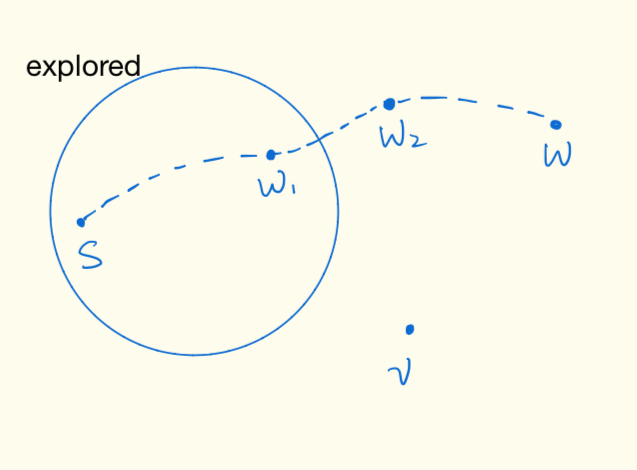
\includegraphics[scale = 0.35]{p1.png}
  \end{center}
  \tab\\
  Denote the subpath from $s$ to $w_1$ in $\Delta(s, w)$ as $p(s, w_1)$, subpath from $s$ to $w_2$ in $\Delta(s, w)$ as $p(s, w_2)$, and subpath $w_2$ to $w$ as $p(w_2, w)$. Based on \texttt{Definition 2.2 Prefix of Path}, $p(s, w_1)$ is a prefix of $\Delta(s, w)$. Since $p(s, w_1)$ is the prefix of the shortest $s-w$ path, then based on \texttt{Lemma 3.1}, $p(s, w_1)$ is the shortest path from $s$ to $w_1$, $\Delta(s, w_1) = p(s, w_1)$, $length(p(s, w_1)) = \delta(w_1)$. 
  \\
  Similarly, since $p(s, w_2) = p(s, w_1) + (w_1, w_2)$, then $p(s, w_2)$ is a prefix of $\Delta(s, w)$, and hence \texttt{Lemma 3.1} implies that $p(s, w_2)$ is the shortest path from $s$ to $w_2$. Then we have: 
  \\\\
  \ftab $\Delta(s, w_2) = p(s, w_2) = p(s, w_1) + (w_1, w_2)$ \\
  \ftab $\delta(w_2) = length(\Delta(s, w_2))$ \\
  \ftab\tab $= length(p(s, w_2))$ \\
  \ftab\tab $= length(p(s, w_1)) + weight(w_1, w_2)$\\
  \ftab\tab $= \delta(w_1) + weight(w_1, w_2)$ ([E1])
  \\
  For $\Delta(s, w)$ we have: 
  \\\\
    \tab\tsp $\delta(w) = length(p_w)$ \\
    \tab\tab $= length(p(s, w_1)) + weight(w_1, w_2) + length(p(w_2, w))$ \\
    \tab\tab $= \delta(w_1) + weight(w_1, w_2) + length(p(w_2, w))$
  \\\\
  Since all edge weights are positive, then: 
  \\\\
    \tab $\delta(w_2) = \delta(w_1) + weight(w_1, w_2) \leq \delta(w)$ ([E2])
  \\\\
  Since $w_1 \in explored_{k+2}$, there are two cases to consider: $w_1 =u_{k+1}$ and $w_1 \neq u_{k+1}$. We will prove P(k+1) under both cases below. 
  \\\\
  \texttt{Case 1: $w_1 = u_{k+1}$}
  \\
  When $w_1 = u_{k+1}$, then substitude $w_1$ by $u_{k+1}$ in [E2], we have: 
  \\\\
    \tab $\delta(w_1) + weight(w_1, w_2) = \delta(u_{k+1}) + weight(u_{k+1}, w_2) \leq delta(w)$\\
    \tab i.e.  $\delta(u_{k+1}) \leq \delta(w)$ 
  \\\\
  which contradicts with our assumption that $\delta(u_{k+1}) > \delta(w)$. Hence by the principle of prove by contradiction, $\delta(u_{k+1}) < \delta(w)$. (1) holds for P(k+1). 
  \\\\
  \texttt{Case 2}: $w_1 \neq u_{k+1}$
  \\ 
  %Since $w_1 \in explored_{k+2}$ and $w_1 \neq v$, $w_1$ is explored before the $(k+1)^{th}$ iteration. i.e., $w_1 \in explored_{k+1}$. Then based on the proof of Part(a) above, $dist_{k+1}[w_1] = \delta(w_1)$. \\

  Since $w_1 \in explored_{k+2}$ and $w_1 \neq u_{k+1}$, $w_1$ is explored before the $(k+1)^{th}$ iteration. i.e., $w_1 \in explored_{k+1}$. Suppose $w_1$ is being explored during the $i^{th}$ iteration, $i < k+1$, then based on the algorithm, the value of $dist_{i+1}[w_1]$ is calculated as: 
  \\\\
  \tab\[
        dist_{i+1}[w_1] = \left.
       \begin{cases} 
          min(dist_{i}[w_1], dist_{i}[w_1] + weight(w_1,w_1)), & (w_1,w_1) \in g \\ 
          dist_{i}[w_1] & otherwise 
        \end{cases}
        \right\}
      \]
  \\\\
  Thus $dist_{i+1}[w_1] = dist_i[w_1]$. Since the inductive hypothesis implies that $dist_{i+1}[w_1] = \delta(w_1)$, then $dist_i[w_1] = \delta(w_1)$. 
  \\
  Since $w_1$ has an edge to $w_2$, then $dist_{i+1}[w_2]$ must have been updated according as follows: 
  \\\\
  \tab\tab $dist_{i+1}[w_2] = min(dist_i[w_2], dist_i[w_1] + weight(w_1 + w_2))$ \\
  \tab\tab\tab $= min(dist_i[w_2], \delta(w_1) + weight(w_1 + w_2))$
  \\\\
  Based on [E1] we know that $\delta(w_2) =  \delta(w_1) + weight(w_1 + w_2)$, then $dist_{i+1}[w_2] = min(dist_i[w_2], \delta(w_2))$. If $dist_i[w_2] = infinity$, then $dist_{i+1}[w_2] = min(dist_i[w_2], \delta(w_2)) = \delta(w_2)$. If $dist_i[w_2] \neq infinity$, then based on \texttt{Lemma 3.2}, $dist_i[w_2]$ is the length of some $s-w_2$ path. Since $\delta(w_2) \leq length(p), \forall p \in path(s, w_2)$, then $dist_{i+1}[w_2] = min(dist_i[w_2], \delta(w_2)) = \delta(w_2)$. Hence in either cases, we conclude that $dist_{i+1}[w_2] = \delta(w_2)$. 
  \\
  Since $dist_{i+1}[w_2] = \delta(w_2)$ and $i < k+1$, then based on \texttt{Lemma 3.3}, we have $dist_{k+1}[w_2] = dist_{i+1} = \delta(w_2)$. Based on [E2], $\delta(w_2) < \delta(w)$, then $dist_{k+1}[w_2] < \delta(w)$ [NE2]. Combining with [NE1], we have: 
  \\\\
  \ftab $\delta(w) < dist_{k+1}[u_{k+1}]$ (from [NE1])\\
  \ftab $dist_{k+1}[w_2] < \delta(w)$ 
  \\\\
  Hence $dist_{k+1}[w_2] < dist_{k+1}[u_{k+1}]$ [NE2]. 
  \\
  Based on our assumption, at the beginning of the $(k+1)^{th}$ generation, $u_{k+1}, w_2 \notin explored_{k+1}$ and $u_{k+1}$ is selected by the algorithm, then we must have $dist_{k+1}[w_2] \geq dist_{k+1}[u_{k+1}]$, which contradicts with [NE2]. Hence by the principle of prove by contradiction, there does not exsist $w \in unexplored_{k+2}$, such that $\delta(u_{k+1}) > \delta(w)$, i.e. $\delta(u_{k+1}) \leq \delta(w), \forall w \in unexplored_{k+2}$. Hence (1) holds for $u_{k+1}$. 
  \\



  \item After the $(k+1)^{th}$ iteration, $dist_{k+1}[u_{k+1}] = \delta(u_{k+1})$
  \\\\
  We will prove this by contradiction. 

  Suppose $dist_{k+1}[u_{k+1}]$ is the length of some path $p$ from $s$ to $u_{k+1}$. Assume the shortest path from $s$ to $u_{k+1}$ is some path different from $p$, i.e. $\Delta(s, u_{k+1}) \neq p$, $\delta(u_{k+1}) \leq dist_{k+1}[u_{k+1}]$([b]). Suppose $v'$ is the node just before $u_{k+1}$ in $\Delta(s, u_{k+1})$. 
  \\\\
  \ftab $\delta(u_{k+1}) = \delta(v') + weight(v', u_{k+1}) < dist_{k+1}[u_{k+1}]$ \\
  \tab\tab\tab Since all edge weights are non-negative, then: $\delta(v') \leq \delta(u_{k+1})$
  \\\\
  Based on (1), after the $(k+1)^{th}$ iteration, for all nodes $q \in unexplored_{k+2}$, $\delta(q) \geq \delta(u_{k+1})$, and $\delta(v') \leq \delta(u_{k+1})$, then $v'$ cannot be in $unexplored_{k+2}$. Since $unexplored_{k+1} = unexplored_{k+2} \cup u_{k+1}$, then $v' \notin unexplored_{k+1}$. Hence at the beginning of the $(k+1)^{th}$ iteration, $v'$ is already explored. Since $v'$ is explored before the $(k+1)^{th}$ iteration and $v'$ has an edge to $u_{k+1}$, then the algorithm must have considered $(\delta(v') + weight(v', u_{k+1}))$ against $dist_{k+1}[u_{k+1}]$ and chose $min((\delta(v') + weight(v', u_{k+1})), dist_{k+1}[u_{k+1}])$, which is $dist_{k+1}[u_{k+1}]$. Thus $dist_{k+1}[u_{k+1}] \leq (\delta(v') + weight(v', u_{k+1}))$, i.e. $dist_{k+1}[u_{k+1}] \leq \delta(u_{k+1})$, which contradicts with our assumption [b]. Hence by the principle of prove by contradiction, $dist_{k+1}[u_{k+1}] = \delta(u_{k+1})$. (2) holds for $u_{k+1}$. 
  \end{enumerate}
\end{itemize}
Since we have proved both (1) and (2) forall nodes in $explored_{k+1}$ after the $(k+1)^{th}$ iteration, P(k+1) holds. Then by the principle of prove by induction, \texttt{Lemma 3.4} holds. 
\end{proof}

\begin{proof}\textbf{Prove of Correctness}
\\\\
By applying \texttt{Lemma 3.4} to the last iteration of the algorithm, we obtained that for all nodes $n$ in the explored list, $dist[n]$ is indeed the shortest path distance value from source $s$ to $n$, hence Dijkstra's algorithm indeed calculates the shortest path distance value from the source $s$ to each node $n \in g$. 
\end{proof}
\end{document}



% \\
% Since during the $(k+1)^{th}$ iteration, $w_1 \in explored_{k+1}$, then $w_1$ must be added into $explored$ with all neighbors of $w_1$ updated during the $i^{th}$ iteration for some $i < k+1$. Then based on our inductive hypothesis, $dist_{i+1}[w_1] = \delta(s, w_1)$. Since for all proceeding $j^{th}$ iterations, $j > i$ the value of $dist_{j+1}$ is calculated by 
% \\\\
%   \tab $dist_{j+1}[w_1] = min(dist_j[w_1], dist_j[q] + weight(q, w_1))$ (if the current node $q$ being explored has an edge $(q, w_1)$ to $w_1$) \\
%   \tab or \\
%   \tab $dist_{j+1}[w_1] = dist_j[w_1]$
% \\\\
% Since $dist_{i+1}[w_1] = \delta(s, w_1) \leq length(p)$ for all path $p$ from $s$ to $w_1$, then for each proceeding $j^{th}$ iteration, there does not exists such $q$ such that $dist_j[q] + weight(q, w_1) < \delta(s, w_1) = dist_{i+1}[w_1]$. Hence $dist[j] = \delta(s, w) = dist_{i+1}s$
% During the $(k+1)^{th}$ iteration, there are two cases: (i) $v$ has an edge to $w_1$; (ii) $v$ does not have an edge to $w_1$. 
% \\
% In \texttt{case (i)}, if $v$ has an edge to $w_1$, then the algorithm must have calculates $dist_{k+1}[w_1]$ as follows: 
% \\\\
%  \tab $dist_{k+1}[w_1] = min(dist_k[w_1], dist_k[v] + weight(v, w_1)) = min(\delta(w_1), dist_k[v] + weight(v, w_1))$
% \\\\
% Based on the definition of shortest path, we must have $\delta(w_1) \leq dist_k[v] + weight(v, w_1)$, hence if $v$ has an edge to $w_1$, we must have $dist_{k+1}[w_1] = \delta(w_1) = dist_k[w_1]$.  
% \\
% In \texttt{case (ii)}, if $v$ does not have an edge to $w_1$, then according to the algorithm, after the $(k+1)^{th}$ iteration, $dist_{k+1}[w_1] = dist_k[w_1] = \delta(w_1)$
% \\
%Since the value of $dist[w_1]$ remains unchanged after adding $w_1$ into $explored$, then $dist_i[w_1] = dist_{k+1}[w_1] = \delta(w_1)$. 



% Since during each iteration the algorithm chooses the node with minimum distance value from the $unexplored$ list, and during the $(k+1)^{th}$ iteration, $w \in unexplored$ and $v \in explored$, then $dist_{k+1}[v] < dist_{k+1}[w]$ holds. 

% Assume $p$ is the $s$ to $v$ path chosen for the $(k+1)^{th}$ iteration, where $dist_{k+1}[v] = length(p)$. Suppose $v'$ is the node right before $v$ in $p$, then $dist_{k+1}[v]$ is updated based on $dist_i[v']$ for some $i \geq 1$, then based on the algorithm, $v'$ must have been explored, hence $i < k+1$, i.e. $i \leq k$, and $v' \in explored$. Since $i \leq k$ and $v' \in explored$, then based on our inductive hypothesis, $\delta(v') = dist_i[v']$. Hence $dist_{k+1}[v] = dist_[v'] + weight(v', v) = \delta(v') + weight(v', v)$. \\
% Based on the definition of shortest path, $\delta(v) \leq dist_{k+1}[v]$ holds. Since $\delta(v) > \delta(w)$, and $\delta(v) \leq dist_{k+1}[v]$, then: 
% \\\\
%  \ftab $\delta(w) < \delta(v)$ \\
%  \ftab $\delta(v) \leq dist_{k+1}[v]$, hence \\
%  \ftab $\delta(w) < dist_{k+1}[v] = \delta(v') + weight(v', v)$\\
% \\\\
% Since all edge weights are positive, then: 
% \\\\
%  \ftab $\delta(w) < dist_{k+1}[v] = \delta(v') + weight(v', v)$\\
%  \ftab $weight(v', v) > 0$ \\
%  \ftab $delta(w) < $
% \\\\
% Since $dist_{k+1}[v] < dist_{k+1}[w]$, and $\delta(v) \leq dist_{k+1}[v]$, then $\delta(v) \leq dist_{k+1}[w]$ holds for the $(k+1)^{th}$ iteration ([a]). 
% \\
% Assume $w'$ is the node just before $w$ in $\Delta(s,w)$(Definition 2.3). Then we have:
% \\\\
% \ftab $\delta(w) = dist[w'] + weight(w', w)$ 
% \\\\
% Since $\delta(w) < \delta(v)$, then: 
% \\\\
% \ftab $\delta(w) < \delta(v)$ \\
% \ftab $dist[w'] + weight(w', w) < \delta(v)$ \\
% \ftab $dist[w'] < \delta(v)$ \\
% \\\\
% Since $dist[w'] < \delta(v)$ and $\delta(v) \leq dist[v]$, then $dist[w'] < dist[v]$. Thus based on the algorithm, the node $w'$ must have been explored before $v$, i.e. $w' \in explored$. Since $w'$ has an edge $(w', w)$ to $w$, then the algorithm must have compared $(dist[w'] + weight(w', w))$ with the current $dist[w]$ before the $k^{th}$ iteration and chose $dist[w]$. Thus it must be $(dist[w'] + weight(w', w)) \geq dist[w]$, i.e. $\delta(w) \geq dist[w]$. Since $\delta(v) > \delta(w)$ and $\delta(w) \geq dist[w]$, then $\delta(v) > dist[w]$, which contradicts with [a]. Hence by the principle of prove by contradiction, (1) holds for the $k^{th}$ iteration. 
% \\